%% Adapted from GaTech CS 7545 Machine Learning Theory given by Prof. Jacob Abernathy Fall 2018. Original latex file: https://github.com/mltheory/CS7545/blob/master/scribe/CS7545scribe_template.tex 



%%%%%PLEASE CONSIDER CORRECTIONS AT PLACES INDICATED%%%%%%%%
\documentclass{article}
%%%%%Packages Used, add more if necessary%%%%
\usepackage{amsmath,amsfonts,amssymb,graphicx,fullpage, float}
\setlength{\topmargin}{-0.6 in}
\setlength{\textheight}{8.5 in}
\setlength{\headsep}{0.75 in}
\usepackage{mdframed}
\usepackage{multicol}
\usepackage{microtype}
\usepackage{hyperref}

%%%%% NO NEED TO EDIT THIS PREAMBLE %%%%%%%%
%%% PREAMBLE %%%
\newcounter{lecnum}
\renewcommand{\thepage}{\thelecnum-\arabic{page}}
\renewcommand{\thesection}{\thelecnum.\arabic{section}}
\renewcommand{\theequation}{\thelecnum.\arabic{equation}}
\renewcommand{\thefigure}{\thelecnum.\arabic{figure}}
\renewcommand{\thetable}{\thelecnum.\arabic{table}}
\newcommand{\lecture}[4]{
   \pagestyle{myheadings}
   \thispagestyle{plain}
   \newpage
   \setcounter{lecnum}{#1}
   \setcounter{page}{1}
   \noindent
   \begin{center}
   \framebox{
      \vbox{\vspace{2mm}
      
      \hbox to 6.28in { 
      {\bf ECE 4252/6252 (FunML) Fundamentals of Machine Learning \hfill 2021--2028} }
      
      \vspace{2mm}
      \hbox to 6.28in { 
      {Courses developed by Professor Ghassan AlRegib 
      (\href{https://alregib.ece.gatech.edu/}{alregib.ece.gatech.edu}) 
      \hfill For inquiries: \href{mailto:alregib@gatech.edu}{alregib@gatech.edu}} }
      
      \vspace{3mm}
      \hbox to 6.28in { {\Large \hfill Lecture #1: #2 \hfill} }
      
      \vspace{2mm}
      \hbox to 6.28in { {\it Co-Instructors: #3 \hfill #4} }
      
      \vspace{2mm}}
   }
   \end{center}

   % -------- PEOPLE OUTSIDE BOX --------
   \vspace{2mm}
   \noindent{\bf Contributors:} Dr. Ahmad Mustafa, Dr. Motaz Alfarraj, Dr. Ashraf Alattar, Dr. Chen Zhou

   \vspace{1mm}
   \noindent{\bf Teaching Assistants} with remarkable contributions include: Kuo-Wei Lai, Wuyang Du, Shiva Mahato, Michael Zhou, Ninghan Zhong

   \markboth{Lecture #1: #2}{Lecture #1: #2}

   \vspace{2mm}
\noindent {\bf Disclaimer}: 
{All content of these notes are part of this course at Georgia Tech. Any re-use or distribution is not permitted without pre-approved permission. All these notes belong to, created by, and copyrighted for Ghassan AlRegib and Mohit Prabhushankar, Georgia Tech, 2021--2028.}

\vspace{2mm}
\noindent {\bf License}: 
{These lecture notes are licensed under the 
\href{https://creativecommons.org/licenses/by-nc-sa/4.0/}{Creative Commons Attribution-NonCommercial-ShareAlike 4.0 International License}.}

   \vspace{2mm}
   \noindent {\bf Errata}: 
   {\it Please submit any errata you find using the following form: 
   \href{https://forms.office.com/r/fbg9dMWPgY}{Errata Form for FunML Textbook} 
   or visit: \url{https://forms.office.com/r/fbg9dMWPgY}}

   \vspace*{4mm}
}
\renewcommand{\cite}[1]{[#1]}
\def\beginrefs{\begin{list}
        {[\arabic{equation}]}{\usecounter{equation}
         \setlength{\leftmargin}{2.0truecm}\setlength{\labelsep}{0.4truecm}%
         \setlength{\labelwidth}{1.6truecm}}}
\def\endrefs{\end{list}}
\def\bibentry#1{\item[\hbox{[#1]}]}

\newcommand{\challenge}[2]{\noindent \textbf{(Challenge Problem)} \emph{#1}: #2 }

\newcommand{\exercise}[1]{\noindent \textbf{(Exercise)} #1 }

\newcommand{\fig}[3]{
			\vspace{#2}
			\begin{center}
			Figure \thelecnum.#1:~#3
			\end{center}
	}
%%% END_OF_PREAMBLE %%%


	
%%%%You may add more \newtheorem if necessary%%%%%%
\newtheorem{theorem}{Theorem}[lecnum]
\newtheorem{lemma}[theorem]{Lemma}
\newtheorem{proposition}[theorem]{Proposition}
\newtheorem{claim}[theorem]{Claim}
\newtheorem{corollary}[theorem]{Corollary}
\newtheorem{definition}[theorem]{Definition}
\newenvironment{proof}{{\bf Proof:}}{\hfill\rule{2mm}{2mm}}


\newcommand{\dom}{\mathrm{dom}}
\begin{document}

%%%%%CHANGE HERE%%%%%%%
%%%%%\section{title of the section} similarly with the rest \section{} or \subsection{} or \subsubsection{} etc


%%%%%CHANGE HERE%%%%%%%%%
%%%%%\lecture{the ordinal number of the lecture}{lecture title}{Jacob Abernethy}{scriber's name}
\lecture{27}{Anomaly Detection}{Ghassan AlRegib and Mohit Prabhushankar}{}

%%%%%CHANGE HERE%%%%%%%
%%%%%\section{title of the section} similarly with the rest \section{} or \subsection{} or \subsubsection{} etc

\section{Lecture Objectives}

This lecture introduces anomaly detection as a machine learning framework for identifying rare, unusual, or unexpected patterns relative to a learned notion of normal behavior. We formalize anomaly detection in a statistical framework by defining anomalies via normal and anomalous data-generating distributions, and by presenting the two core components of a detector: a statistic (or anomaly score) and a decision rule (typically thresholding). We then develop evaluation methodology for anomaly detection under class imbalance, including TPR, FPR, precision, ROC curves, and AUC, and we analyze how the decision threshold controls the trade-off between missed detections and false alarms. Next, we study two practical learning settings---semi-supervised (novelty detection) and unsupervised anomaly detection---highlighting their assumptions and representative techniques such as density-based detection, distance-based methods, and Isolation Forest. Finally, we focus on image anomaly detection methods, including patch-based statistical modeling, adjacent pixel-value correlation structure, and neural network-based confidence scoring via Maximum Softmax Probability (MSP), and we connect these ideas to the manifold hypothesis and reconstruction-based approaches (e.g., autoencoders), including gradient-based regularization such as GradCON and hybrid/ensemble strategies for robust detection in high-dimensional settings.

\section{Anomaly Detection}

Anomaly detection refers to a class of machine learning techniques designed to identify rare, unusual, or unexpected patterns that deviate from a learned notion of normal behavior. Rather than focusing on predicting predefined labels, anomaly detection aims to model what is considered “normal” and then flag observations that significantly differ from this model. Although anomaly detection is not a standalone application domain, it plays a crucial role across many fields, including fraud detection, medical diagnosis, cybersecurity, industrial monitoring, and fault detection. In this lecture, we introduce the anomaly detection framework and discuss its core components, including the formal definition of anomalies, problem formulation, evaluation metrics, different anomaly detection settings, statistical approaches, reconstruction-based approaches, and the GradCON method.

\subsection{Definition}

An anomaly (also referred to as an outlier or novelty) is a data point or pattern that deviates significantly from the expected distribution of normal data. More formally, anomaly detection involves learning a model of normal data and identifying samples that have low likelihood or high deviation relative to this learned model. The central challenge lies in defining and modeling “normality,” since anomalies are inherently rare and often diverse in nature.

In a probabilistic framework, we assume that normal data are generated from an underlying distribution $P_N$. Anomalies can then be interpreted as observations that are unlikely under $P_N$, or equivalently, as samples that may originate from a different distribution $P_A$, where $P_A \neq P_N$. Importantly, anomalies do not necessarily arise from non-stationary processes; rather, they correspond to deviations from the dominant data-generating process. In many practical settings, $P_A$ is unknown, poorly sampled, or highly heterogeneous, which makes anomaly detection particularly challenging.

In time-series contexts, normal behavior is sometimes modeled as a stationary process (with stable statistical properties such as mean and variance). However, anomalies may appear either as rare realizations within a stationary system or as changes in the underlying generating mechanism. Therefore, anomaly detection is fundamentally about distinguishing rare or structurally inconsistent observations from the learned representation of normal data, regardless of whether the deviation arises from distributional shift, structural corruption, or unexpected dynamics.

\subsection{Examples of Anomaly Detection}

Anomaly detection appears in a wide range of real-world applications where rare but critical events must be identified within large volumes of normal data. One common example is fraud detection in financial systems, where the goal is to identify suspicious transactions within streams of otherwise normal credit card activity. Another important application arises in healthcare, where anomaly detection is used to identify arrhythmias in electrocardiogram (ECG) signals that deviate from typical heart rhythms. In computer vision, anomaly detection can be used to locate defective regions in images that do not conform to a reference pattern, such as manufacturing defects in materials or unexpected objects in surveillance footage.

A key observation across these domains is that anomalies often appear as spurious or irregular elements embedded within structured data. Although anomalous samples are typically rare, they are often the most informative and valuable data points in a dataset because they highlight unusual behavior, critical failures, or events of interest that require further investigation.

Figure~\ref{fig:anomaly_material_example} illustrates an example of structural anomalies within a material, where irregular regions deviate from an otherwise consistent pattern. Such defects are often subtle and difficult to detect manually, motivating automated anomaly detection techniques.

\begin{figure}[H]
    \centering
    
\includegraphics[width=0.5\linewidth]{img/lecture24/image1.png}
    \caption{Example of anomalous structures within a structured material.}
    \label{fig:anomaly_material_example}
\end{figure}

Anomaly detection is also widely used in public safety and surveillance scenarios. Figure~\ref{fig:anomaly_surveillance_example} shows an example in which an unusual individual is detected within a crowd. In such settings, anomaly detection systems help identify unusual or suspicious behavior in large-scale visual data.

\begin{figure}[H]
    \centering
    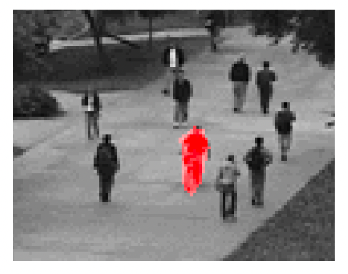
\includegraphics[width=0.5\linewidth]{img/lecture24/Picture2.png}
    \caption{Anomaly detection scenario in a public setting.}
    \label{fig:anomaly_surveillance_example}
\end{figure}


\subsection{Anomaly Detection in Images}

To study anomaly detection in images, we first formulate the problem mathematically. 
Let $s$ denote an image defined over a discrete pixel domain $x \in \mathbb{Z}^2$. 
For a specific pixel location $c \in x$, the value $s(c)$ represents the image 
intensity (or feature value) at that pixel.

The goal of image anomaly detection is to identify pixels or regions that deviate 
from normal image structure. This task can be expressed through the estimation of 
an anomaly mask $\Omega$, which assigns a binary label to each pixel:
\begin{equation}
  \Omega(c)=
  \begin{cases}
    0, & \text{if pixel $c$ belongs to a normal region},\\
    1, & \text{if pixel $c$ belongs to an anomalous region}.
  \end{cases}
\end{equation}

While this formulation focuses on images, anomaly detection is often studied in a 
more general setting where observations are collected over time. Consider a set of 
data samples represented as $\{x(t)\}_{t=t_0}^{T}$, where each observation 
$x(t) \in \mathbb{R}^d$. These samples are assumed to be generated by an underlying 
probabilistic process. In the normal case, data are drawn from a distribution 
$\phi_0$, which represents typical or expected behavior.

Anomaly detection then reduces to identifying observations that deviate 
significantly from this normal distribution. A simple generative model assumes that 
each observation is produced by one of two distributions:
\begin{equation}
  x(t) \sim
  \begin{cases}
    \phi_0, & \text{if $x(t)$ belongs to normal data},\\
    \phi_1, & \text{if $x(t)$ belongs to anomalous data}.
  \end{cases}
\end{equation}

Under this perspective, anomaly detection becomes the task of distinguishing 
samples generated by the normal distribution $\phi_0$ from those generated by an 
alternative distribution $\phi_1$. This probabilistic view unifies anomaly detection 
across images, time series, and high-dimensional data.

\subsection{Anomaly Detection in a Statistical Framework}

A classical approach to anomaly detection is based on statistical hypothesis
testing. The core idea is to monitor data using a \emph{statistic} that behaves
predictably under normal conditions and to trigger an alarm when the statistic
deviates significantly from this expected behavior.

In this framework, anomaly detection consists of two fundamental components:
(1) a statistic that summarizes the behavior of the data, and  
(2) a decision rule that determines whether the observed behavior is considered
normal or anomalous.

Figure~\ref{fig:anomaly_timeseries_process} illustrates this idea for a
time-series signal: most observations are generated by a normal process
$\phi_0$, while occasional samples arise from an anomalous process $\phi_1$.

\begin{figure}[H]
    \centering
    
\includegraphics[width=0.5\linewidth]{img/lecture24/Picture3.png}
    \caption{Process of detecting anomalies in a time-series signal $x(t)$}
    \label{fig:anomaly_timeseries_process}
\end{figure}

\subsubsection{Statistics}

A \emph{statistic} is a numerical quantity computed from data that summarizes
its behavior. Under normal operating conditions, the statistic follows a
predictable distribution, and significant deviations from this expected
behavior may indicate anomalous data. 

Typical statistics used in anomaly detection include the sample mean or moving average, the sample variance or signal energy, log-likelihood values under a probabilistic model, classifier confidence scores, and learned \emph{anomaly scores} designed specifically to highlight deviations from normal patterns. 

The key objective is to select a statistic that remains stable for normal data while being sensitive to unusual or unexpected observations.

\subsubsection{Decision Rule}

The \emph{decision rule} converts the statistic into a binary decision:
\[
\text{Normal} \quad \text{vs.} \quad \text{Anomalous}.
\]
This is typically done by comparing the statistic to a threshold or confidence
region derived from normal data.

Two common decision strategies are:

\begin{itemize}
\item \textbf{Threshold-based detection:}  
An observation is flagged as anomalous if the statistic exceeds a threshold
$\gamma$, i.e.,
\[
S(x) > \gamma.
\]

\item \textbf{Confidence-region detection:}  
Normal data are assumed to lie within a region of high probability under the
normal model. Observations outside this region are considered anomalies.
\end{itemize}

Figure~\ref{fig:statistical_anomaly_detection} illustrates the
\emph{threshold-based detection} strategy. As the statistic evolves over time,
an anomaly is declared when it crosses the decision threshold $\gamma$.

\begin{figure}[H]
    \centering
    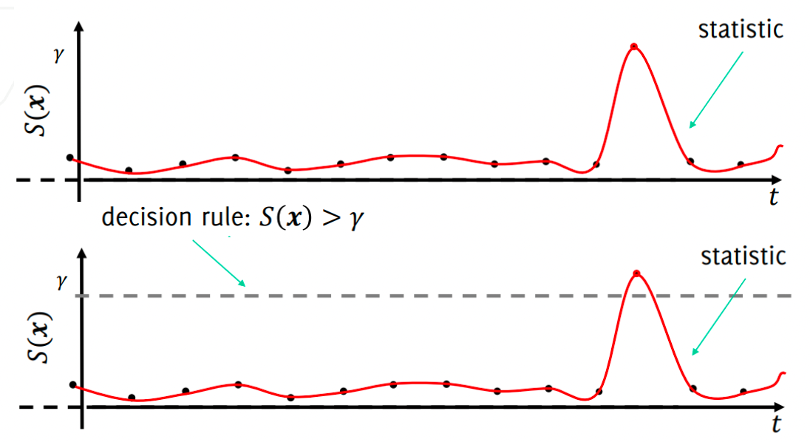
\includegraphics[width=0.5\linewidth]{img/lecture24/Picture4.png}
    \caption{Threshold-based anomaly detection: an evolving statistic crosses the
decision threshold $\gamma$, triggering an anomaly alarm.}
    \label{fig:statistical_anomaly_detection}
\end{figure}

\subsection{Performance Metrics}

When applying anomaly detection, it is essential to clearly define the
evaluation objective. In many real-world scenarios, anomaly detection is
formulated as a \textbf{binary classification problem} in which each sample is
classified as either \emph{normal} or \emph{anomalous}. In contrast to standard
classification settings, anomaly detection typically involves
\textbf{extreme class imbalance}, since anomalous events are rare compared to
normal observations. As a result, accuracy alone is often insufficient, and
specialized metrics are required to properly evaluate performance.

\subsubsection{True Positive Rate and False Positive Rate}

Two fundamental performance measures are the \textbf{True Positive Rate (TPR)}
and the \textbf{False Positive Rate (FPR)}.

% \paragraph{True Positive Rate (TPR)}
\hspace{4cm}

The \textbf{True Positive Rate} measures how many anomalies are correctly
detected:

\begin{equation}
\text{TPR} = \frac{\text{number of anomalies correctly detected}}
{\text{total number of anomalies}}
\end{equation}

TPR is also known as \emph{recall}, \emph{sensitivity}, or the \emph{hit rate}.
It reflects the ability of the algorithm to successfully identify anomalous
samples.

% \paragraph{False Positive Rate (FPR)}
\hspace{4cm}

The \textbf{False Positive Rate} measures how often normal data are incorrectly
flagged as anomalies:

\begin{equation}
\text{FPR} = \frac{\text{number of normal samples incorrectly flagged as anomalies}}
{\text{total number of normal samples}}
\end{equation}

A high FPR indicates many false alarms, which may be costly or disruptive in
practice.

From previous lectures, recall that the remaining related metrics are

\[
\text{FNR} = 1 - \text{TPR}, \qquad
\text{TNR} = 1 - \text{FPR}.
\]

We also define the \textbf{precision on anomalies} as

\begin{equation}
\text{Precision} =
\frac{\text{number of anomalies correctly detected}}
{\text{total number of detected anomalies}}.
\end{equation}

\subsubsection{Threshold Trade-off}

Most anomaly detection systems rely on a decision threshold $\gamma$ applied to
a statistic $S(x)$. Changing this threshold directly affects performance.

\begin{itemize}
\item Lower threshold $\gamma$: increases TPR but may increase FPR
      (more false alarms).
\item Higher threshold $\gamma$: decreases FPR but may reduce TPR
      (more missed anomalies).
\end{itemize}

Figure~\ref{fig:anomaly_threshold_tradeoff} illustrates how changing the
decision threshold affects detection.

\begin{figure}[H]
\centering
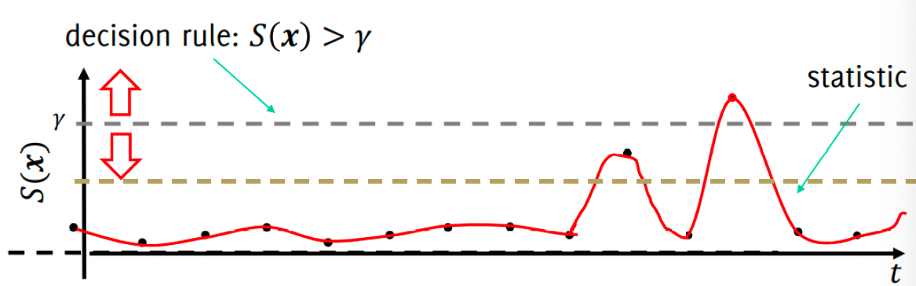
\includegraphics[width=0.5\linewidth]{img/lecture24/Picture24.5.png}
\caption{Effect of the decision threshold on anomaly detection. Lower thresholds detect more anomalies but increase false positives, while higher thresholds reduce false positives but may miss anomalies.}
\label{fig:anomaly_threshold_tradeoff}
\end{figure}

\subsubsection{Combined Performance Metrics}

Because TPR and FPR capture different aspects of performance, it is common to
use metrics that combine multiple quantities.

\paragraph{Accuracy}

\begin{equation}
\text{Accuracy} =
\frac{\text{TP} + \text{TN}}{\text{Total samples}}
\end{equation}

Accuracy measures overall correctness, but can be misleading when anomalies are
rare.

\paragraph{F1 Score}

\begin{equation}
\text{F1} =
\frac{2 \cdot \text{Precision} \cdot \text{Recall}}
{\text{Precision} + \text{Recall}}
\end{equation}

The F1 score balances precision and recall and is widely used in anomaly
detection because it accounts for both missed anomalies and false alarms.

In an ideal detector, all anomalies are detected with no false positives,
resulting in maximum values for both accuracy and F1 score.

\subsubsection{Area Under the Curve (AUC)}

Comparing anomaly detection algorithms using a single threshold can be misleading,
since different applications may require different trade-offs between missed
anomalies and false alarms. To evaluate performance across all possible decision
thresholds, we use the \emph{Receiver Operating Characteristic (ROC) curve}.

The ROC curve plots the \emph{True Positive Rate (TPR)} against the
\emph{False Positive Rate (FPR)} while sweeping the decision threshold $\gamma$.
Each point on the curve corresponds to a specific threshold choice.

An ideal detector would achieve
\[
\text{FPR} = 0, \qquad \text{TPR} = 1,
\]
which corresponds to the top-left corner of the ROC plot. In practice,
a detector is considered better when its ROC curve lies closer to this corner.

The \emph{Area Under the Curve (AUC)} summarizes the ROC curve into a single
scalar value:
\begin{itemize}
\item A higher AUC indicates better overall discrimination between normal and anomalous data.
\item An AUC of $1$ represents perfect detection.
\item An AUC of $0.5$ corresponds to random guessing.
\end{itemize}

Figure~\ref{fig:roc_auc_anomaly} shows ROC curves for several anomaly detection
methods. Each curve corresponds to a different algorithm, and the associated
AUC values allow direct quantitative comparison.

\begin{figure}[H]
    \centering
    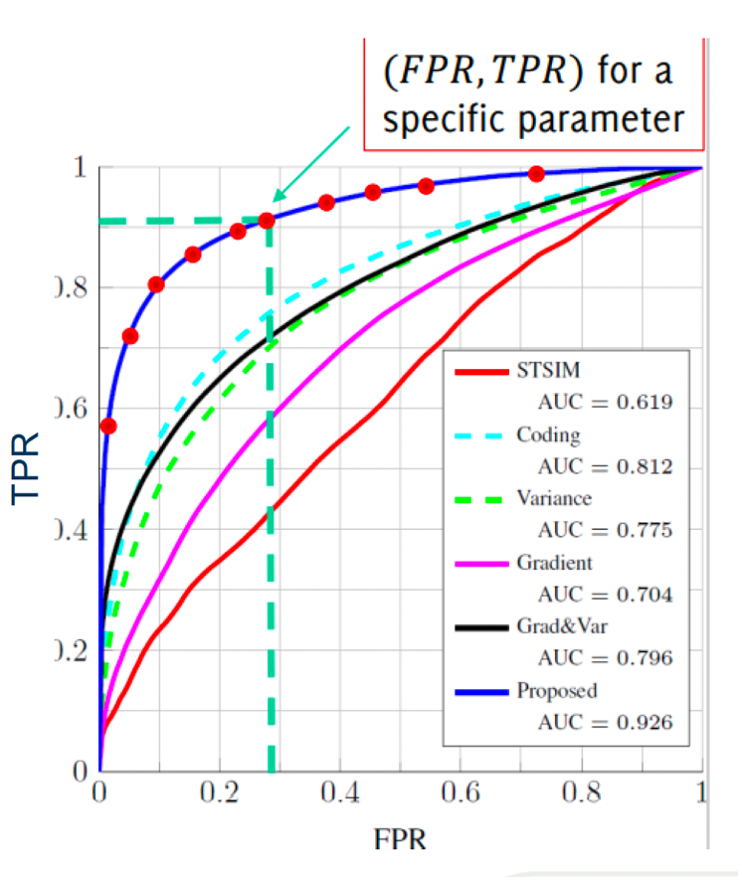
\includegraphics[width=0.5\linewidth]{img/lecture24/Picture6.png}
    \caption{ROC curve comparison across anomaly detection methods.  
    Curves closer to the top-left corner and with larger AUC values indicate
    superior detection performance.}
    \label{fig:roc_auc_anomaly}
\end{figure}

Overall, ROC curves and AUC provide a robust and threshold-independent framework
for evaluating and comparing anomaly detection algorithms.

% \exercise{The professor mentioned an exercise in class that would be useful to work out. You can use the \texttt{$\backslash$exercise} command in these cases.}

% \challenge{Name of Challenge Problem}{If a challenge problem is given out, give it a name and put it in the previous field and then write down the description in this field.}


\section{Anomaly Detection Settings}

Anomaly detection can be formulated under three primary learning settings,
depending on the availability of labeled data. 

In the \textbf{semi-supervised}
setting, the training data consists primarily of normal examples, and the model
learns a representation of normal behavior in order to flag deviations at test
time. 

In the \textbf{unsupervised} setting, no labels are available at all; the
algorithm must discover unusual patterns directly from the data distribution,
which may contain a mixture of normal and anomalous samples. 

In the \textbf{supervised} setting, labeled examples of both normal and anomalous data
are provided, allowing the task to be treated as a standard binary classification problem.

\subsection{Semi-supervised Anomaly Detection}

Semi-supervised anomaly detection assumes that the training set contains
primarily \emph{normal} data. The goal is therefore to learn a model of normal
behavior and detect deviations at test time.

\subsubsection{Context and Assumptions}

Let the training set be
\[
\mathcal{T}_R = \{x(t)\mid x(t)\sim \phi_0,\; t < t_0\},
\]
where $\phi_0$ denotes the distribution of normal data.

This setting relies on several key assumptions. First, normal data are abundant
and relatively easy to collect. In contrast, anomalous data are rare, costly,
and difficult to label, making it unrealistic to obtain a representative set of
all possible anomalies. Consequently, the training set may contain little or no
anomalous data. For this reason, semi-supervised anomaly detection is often
referred to as \emph{novelty detection}.

\subsubsection{Density-based Detection}

A natural strategy is to model what \emph{normal data look like} and treat
unlikely observations as anomalies. This leads to density-based methods, which
estimate the probability density of normal data and monitor how likely new
observations are under this model.

\paragraph{Training phase.}  
Estimate the probability density function $\phi_0$ using the normal training
data. A typical choice is a Gaussian Mixture Model (GMM), which represents the
distribution as a weighted combination of Gaussian components.

\paragraph{Testing phase.}  
For each incoming sample, compute its log-likelihood under the learned model:
\[
L(x(t))=\log \phi_0(x(t)).
\]
The sequence $\{L(x(t))\}_{t=1}^{\infty}$ is then monitored over time. Samples
with unusually low likelihood are flagged as anomalies.

In practice, this is implemented by comparing $L(x(t))$ to a threshold
$\gamma$, declaring an anomaly when $L(x(t)) < \gamma$.

If anomalous data receive high likelihood under the model, this indicates that
the chosen statistic or density model is not sufficiently discriminative.

\subsubsection{Advantages and Limitations}

\paragraph{Advantages.}  
The learned density $\phi_0$ provides a probabilistic confidence measure,
analogous to a p-value. Robust estimators can tolerate a small fraction of
anomalies in the training set.

\paragraph{Limitations.}  
Density estimation becomes challenging in high-dimensional spaces due to the
curse of dimensionality, leading to high computational cost and risk of
overfitting.

\subsection{Unsupervised Anomaly Detection}

Unsupervised anomaly detection assumes that no labels are available during
training. In contrast to semi-supervised settings, the training set may contain
both normal and anomalous samples, but their identities are unknown. The goal
is therefore to identify observations that deviate from the dominant structure
of the data without prior knowledge of what constitutes an anomaly.

\subsubsection{Context and Assumptions}

Let the training set be
\[
\mathcal{T}_R = \{x(t) \mid t < t_0\},
\]
where $x(t)$ denotes an observation collected at time $t$.

In this setting, both normal and anomalous samples may be present in
$\mathcal{T}_R$, but no labels are provided. A central assumption underlying
most unsupervised methods is that anomalies are rare relative to normal data.
Consequently, the majority of observations reflect regular behavior, while
anomalies appear as statistical or structural deviations from this majority.

Because no labeled validation data are available, many unsupervised algorithms
produce continuous \emph{anomaly scores} rather than binary decisions. Final
anomaly labels are obtained by applying a threshold to these scores, making
unsupervised anomaly detection naturally formulated as a ranking problem.

\subsubsection{Detection Strategies}

Without labeled normal data, the strategy shifts from explicitly modeling
normality to identifying structural irregularities in the dataset. Broadly
speaking, unsupervised methods rely on one of the following principles:

Normal data tend to cluster together, occupy dense regions of the feature
space, and require many operations to isolate. In contrast, anomalous samples
often lie far from dense clusters, reside in sparse regions, or are easier to
separate from the rest of the data.

We discuss two widely used approaches below.

\subsubsection{Distance-Based Methods}

Distance-based methods assume that normal observations lie in dense
neighborhoods, whereas anomalies are relatively distant from their nearest
neighbors.

\begin{figure}[H]
    \centering
    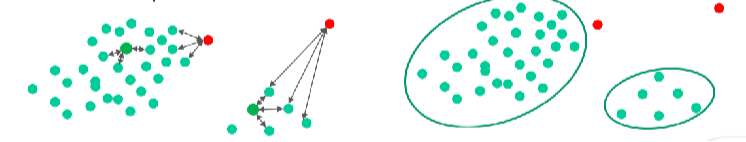
\includegraphics[width=0.75\linewidth]{img/lecture24/Picture1.png}
    \caption{Distance-based anomaly detection: anomalies lie far from dense clusters.}
    \label{fig:distance_based}
\end{figure}

Under this approach, each data point is assigned an anomaly score based on its
distance to nearby samples.

\paragraph{Algorithm overview.}
\begin{enumerate}
    \item For each data point, compute its distance to the $k$ nearest neighbors.
    \item Estimate local sparsity by aggregating these distances.
    \item Assign larger anomaly scores to points with unusually large distances.
    \item Declare anomalies by thresholding the resulting scores.
\end{enumerate}

The performance of distance-based methods depends strongly on the choice of
distance metric and the parameter $k$. These approaches may become
computationally expensive for large datasets and can suffer in high-dimensional
spaces where distances become less informative.

\subsubsection{Isolation Forest}

Isolation Forest adopts a different perspective based on the observation that
anomalies are both rare and different, making them easier to isolate.

Instead of measuring distances or densities, the algorithm constructs an
ensemble of randomly generated binary trees that recursively partition the
feature space. Because anomalous samples are unusual, they tend to be isolated
in fewer partitioning steps than normal data points.

\begin{figure}[H]
    \centering
    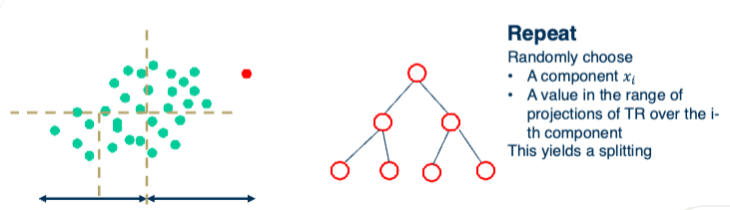
\includegraphics[width=0.5\linewidth]{img/lecture24/Picture8.png}
    \caption{Isolation Forest: anomalies are isolated in fewer splits.}
    \label{fig:isolation_forest}
\end{figure}

\paragraph{Algorithm overview.}
\begin{enumerate}
    \item Randomly select a feature and a split value within its range.
    \item Recursively partition the data to form isolation trees.
    \item Measure the path length required to isolate each sample.
    \item Assign higher anomaly scores to samples with shorter path lengths.
\end{enumerate}

Isolation Forest is computationally efficient, scales well to high-dimensional
datasets, and requires relatively few assumptions about the underlying data
distribution.

\subsubsection{Advantages and Limitations}

\paragraph{Advantages.}
Unsupervised methods do not require labeled data, making them practical in
domains where anomalies are rare or difficult to annotate. They are flexible
and can be applied across a wide range of applications, including cybersecurity,
industrial monitoring, and financial fraud detection.

\paragraph{Limitations.}
Because no labels are available, model selection and hyperparameter tuning are
more challenging than in supervised settings. Many methods rely on the
assumption that anomalies are rare, which may not always hold. In addition,
high-dimensional data can degrade performance due to the curse of
dimensionality. Finally, interpreting anomaly scores and explaining why a
sample is considered anomalous remains a significant challenge.

\section{Statistical Methods}

Image-based anomaly detection aims to identify regions of an image that deviate
from expected visual patterns. In many practical applications, anomalies are
localized rather than global. For example, a manufacturing defect may appear as
a small scratch on a surface, and a medical abnormality may occupy only a small
region of a scan. Treating the entire image as a single data point may therefore
hide subtle but important irregularities.

To address this limitation, statistical approaches often operate at the level
of \emph{image patches}. By analyzing smaller regions independently, the model
can detect localized deviations while still capturing the global distribution
of normal visual patterns.

\subsection{Patch-based Image Analysis}

Patch-based image analysis divides each image into smaller regions, called
\emph{patches}. These patches may be non-overlapping or overlapping depending on
the desired spatial resolution. Each patch is treated as an individual sample
drawn from the distribution of normal image regions.

This approach converts the anomaly detection problem into a statistical density
estimation task: learn the distribution of normal patches during training, and
identify patches that are unlikely under this learned distribution during
testing.

\subsubsection{Training Process}

During training, the model observes only normal images and learns the
statistical distribution of their patches.

\begin{enumerate}
    \item Normal training images are divided into patches $s$ of fixed size
    (for example $4\times4$ or $8\times8$ pixels). Each patch is reshaped into a
    feature vector.
    
    \item The distribution of normal patches is modeled using a multivariate
    Gaussian distribution
    \[
        \phi_0(s) = \mathcal{N}(\mu,\Sigma),
    \]
    where $\mu$ is the mean vector and $\Sigma$ is the covariance matrix
    estimated from all normal training patches.
    
    \item The learned distribution $\phi_0$ provides a probabilistic model of
    what normal image regions look like and allows us to evaluate how likely a
    new patch is under normal conditions.
\end{enumerate}

\subsubsection{Testing Process}

During inference, new images are analyzed patch-by-patch and compared to the
learned normal distribution.

\begin{enumerate}
    \item Each test image is divided into patches using the same procedure as in
    training.
    
    \item For every patch $s$, the likelihood $\phi_0(s)$ (or equivalently the
    log-likelihood $\log\phi_0(s)$) is computed.
    
    \item Patches whose likelihood falls below a predefined threshold are
    classified as anomalous.
\end{enumerate}

By aggregating anomaly scores across patches, a heatmap can be produced that
highlights anomalous regions within the image.

\subsubsection{Challenges}

Although conceptually simple, patch-based Gaussian modeling faces several
practical challenges.

First, increasing the patch size dramatically increases the dimensionality of
the feature space. A patch of size $k\times k$ produces a $k^2$-dimensional
vector, making covariance estimation difficult and computationally expensive.
This phenomenon is a manifestation of the \emph{curse of dimensionality}.

Second, neighboring patches in real images are not independent. Natural images
contain spatial structure and correlations that simple Gaussian models fail to
capture. Ignoring these dependencies can reduce detection accuracy.

Finally, modeling raw pixel intensities assumes that pixel distributions are
approximately Gaussian, which is often unrealistic. Modern approaches therefore
extend this framework using learned feature representations from deep neural
networks, which provide more robust and semantically meaningful patch
descriptors.

\subsection{Adjacent Pixel-value Distribution}

While patch-based Gaussian modeling treats each patch as a vector of pixel
intensities, it often ignores an important property of natural images:
\emph{spatial correlation}. Adjacent pixels in real-world images are not
independent. Instead, they exhibit strong dependencies due to smooth transitions,
edges, textures, and structured patterns.

Understanding these spatial relationships is crucial for effective anomaly
detection, as anomalies often disrupt the natural correlation structure of an
image.

\subsubsection{Correlation in Spatial Data}

In natural images, neighboring pixel intensities tend to vary gradually rather
than abruptly. This smoothness creates strong correlations between adjacent
pixels. For example, in a uniform region, neighboring pixels typically have
similar intensity values, while along edges, structured directional changes
appear.

Modeling such dependencies using simple probabilistic assumptions—such as a
multivariate Gaussian distribution with independent components—is often
insufficient. Even when covariance matrices are included, Gaussian models may
struggle to capture the complex, nonlinear relationships present in spatial
image data.

\subsubsection{Statistical Insights}

One way to visualize spatial dependencies is through histograms and scatter
plots of adjacent pixel intensities. For instance, plotting the intensity of a
pixel against that of its neighbor often reveals concentrated patterns along
structured regions, reflecting underlying correlations.

In normal images, these scatter plots exhibit consistent structures. Anomalies,
however, tend to distort these patterns, appearing as deviations from the
typical distribution of neighboring pixel values.

This observation highlights a limitation of simple Gaussian patch models:
as patch dimensionality increases, covariance estimation becomes unstable and
insufficient to capture the full complexity of spatial dependencies,
particularly in highly textured or structured regions.

\subsubsection{Implications for Anomaly Detection}

Because pixel correlations encode important structural information, ignoring
them can reduce detection sensitivity. Anomalies may not significantly change
individual pixel intensities, but they can disrupt local spatial consistency.

Effective anomaly detection methods therefore need to account for local pixel
interactions. This motivates more advanced techniques—such as convolutional
filters in neural networks—that explicitly model spatial structure and learn
hierarchical representations of texture and shape.

Incorporating adjacent pixel relationships enhances robustness and improves
the ability to detect subtle, localized anomalies that may not be evident from
independent pixel statistics alone.

\subsection{Maximum Softmax Probability (MSP)}

Maximum Softmax Probability (MSP) is a simple yet influential neural
network–based technique for anomaly detection and out-of-distribution (OOD)
detection. Rather than building a separate anomaly detector, MSP leverages the
probability outputs of an existing classification model. The key intuition is
that a well-trained classifier should produce confident predictions for
in-distribution samples and lower confidence for unfamiliar or anomalous inputs.

\begin{figure}[H]
    \centering
    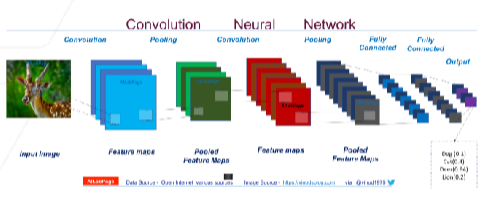
\includegraphics[width=0.5\linewidth]{img/lecture24/Picture10.png}
    \caption{Using a trained convolutional neural network for anomaly detection via softmax confidence.}
    \label{fig:msp}
\end{figure}

\subsubsection{Concept and Motivation}

Modern neural networks trained for classification typically end with a
\emph{softmax layer} that converts logits into class probabilities:
\[
p(y=c \mid x)=\frac{\exp(z_c)}{\sum_j \exp(z_j)}.
\]
These probabilities represent the model's confidence that an input belongs to
each class.

The central idea behind MSP is that the \emph{maximum} softmax probability
reflects the model's confidence in its prediction:
\[
\text{MSP}(x)=\max_c p(y=c\mid x).
\]
For inputs drawn from the training distribution, the model typically assigns a
high probability to one class. In contrast, anomalous or OOD inputs often lead
to uncertain predictions, resulting in lower maximum softmax probabilities.

Therefore, anomaly detection can be reframed as a \emph{confidence estimation}
problem.

\subsubsection{Methodology}

MSP performs anomaly detection by applying thresholding to the confidence score
produced by the classifier. After training a model on in-distribution data, the
maximum softmax probability is computed for each test sample. A threshold
$\gamma$ is then chosen to separate normal and anomalous inputs:
\[
\text{Declare anomaly if } \text{MSP}(x) < \gamma.
\]

This procedure does not require retraining or modifying the classifier.
Instead, anomaly detection is implemented as a lightweight post-processing
step. In practice, the threshold is selected using validation data to balance
false positives and false negatives.

The method implicitly distinguishes between \emph{in-distribution} and
\emph{out-of-distribution} samples. In-distribution inputs typically produce a
peaked probability distribution dominated by one class, whereas OOD inputs tend
to produce flatter distributions because the network has not learned
representations for them.

\subsubsection{Advantages}

MSP is widely used because of its simplicity and practicality. It can be applied
to any trained classifier without changing the training procedure or network
architecture. This makes it computationally efficient and easy to deploy in
real-world systems. The method is also model-agnostic and can be applied to
convolutional networks, transformers, and other modern architectures.

Despite its simplicity, MSP often provides a surprisingly strong baseline for
OOD detection and is commonly used as a benchmark when evaluating more advanced
methods.

\subsubsection{Limitations and Challenges}

Although effective, MSP has important limitations. Neural networks can be
\emph{overconfident} on unfamiliar inputs, sometimes assigning high softmax
probabilities to samples that are clearly out of distribution. This phenomenon
is related to the calibration of neural networks and their tendency to produce
poorly calibrated probability estimates.

Performance also depends strongly on the choice of threshold, which may vary
across datasets and deployment environments. Furthermore, MSP relies solely on
output probabilities and does not exploit internal feature representations of
the network, which can contain richer information for anomaly detection.

These limitations have motivated the development of more advanced techniques,
such as temperature scaling, energy-based models, and feature-based OOD
detection methods.

\subsection{Manifolds in Natural Images}

A fundamental insight underlying modern anomaly detection in vision is the
\emph{manifold hypothesis}. Although images are represented in very
high-dimensional spaces—for example, a $256\times256$ RGB image lies in
$\mathbb{R}^{196{,}608}$—natural images do not occupy this space uniformly.
Instead, they concentrate near a much lower-dimensional structure known as a
\emph{data manifold}.

Intuitively, natural images are governed by underlying physical and semantic
constraints: lighting conditions, object shapes, textures, and spatial
continuity. These constraints dramatically reduce the degrees of freedom of
valid images. As a result, normal image patches lie close to a low-dimensional
manifold embedded in the ambient high-dimensional pixel space.

Anomalies, in contrast, correspond to samples that deviate from this manifold.
They may violate structural consistency, introduce unusual textures, or break
the statistical regularities that characterize normal data. In geometric terms,
anomalous samples lie farther away from the learned manifold of normal images.

\subsubsection{Geometric Interpretation}

Let $\mathcal{M}$ denote the manifold representing normal image data.
Under the manifold hypothesis, in-distribution samples satisfy
\[
x \approx \mathcal{M},
\]
meaning they lie near the manifold. Anomalies satisfy
\[
\text{dist}(x, \mathcal{M}) \text{ is large},
\]
where $\text{dist}(\cdot,\mathcal{M})$ measures the distance to the manifold.

Anomaly detection can therefore be interpreted as estimating how far a sample
deviates from the learned low-dimensional structure of normal data.

\subsubsection{Connection to Neural Networks}

Deep neural networks, particularly Convolutional Neural Networks (CNNs),
implicitly learn representations that capture this manifold structure.
Instead of operating directly in raw pixel space, CNNs map images into
lower-dimensional latent feature spaces where normal samples tend to cluster
together.

In these latent spaces, the manifold structure becomes more explicit.
Normal data form compact clusters or smooth regions, while anomalous inputs
often appear as outliers. This explains why feature-based anomaly detection
methods—such as reconstruction error in autoencoders or distance-based methods
in embedding space—are often more effective than methods applied directly to
pixels.

By leveraging learned feature representations, modern anomaly detection systems
approximate the underlying manifold and identify deviations from it. This
geometric perspective provides both interpretability and improved detection
precision in complex, high-dimensional datasets.

\subsection{Hybrid and Reconstruction-Based Methods}

The methods presented so far each capture different aspects of abnormal
behavior. In practice, modern anomaly detection systems often combine
statistical modeling, manifold learning, and deep learning in order to
overcome the limitations of individual approaches. A particularly important
family of techniques is based on \emph{reconstruction}, which assumes that a
model trained only on normal data will learn to accurately reproduce normal
patterns while failing to reconstruct anomalous inputs.

\subsubsection{Reconstruction-Based Detection}

Reconstruction-based methods learn a model $\mu$ that captures the structure
of normal observations. Instead of directly modeling anomaly likelihood, the
approach detects anomalies through the \emph{reconstruction error}, i.e., the
difference between an input and its reconstruction. The key intuition is that
a model trained exclusively on normal data can reconstruct normal samples well,
whereas anomalous inputs produce large residual errors.

\paragraph{Training phase.}
Given a training dataset $\mathcal{T}_R$ consisting of normal samples, the model
$\mu$ is trained to encode and reconstruct the input signal. The objective is
to minimize a reconstruction loss that encourages the model to capture the
dominant structure of the normal data distribution.

\paragraph{Testing phase.}
At test time, each new observation $s$ is passed through the trained model to
produce a reconstruction $\hat{s}=\mu(s)$. The anomaly score is computed from
the residual error
\[
\mathrm{err}(s)=\|s-\mu(s)\|.
\]
Samples with unusually large reconstruction errors are flagged as anomalies.
In practice, detection is performed by comparing the reconstruction error to
a threshold $\gamma$ learned from validation data.

\subsubsection{Autoencoders as a Canonical Example}

Autoencoders provide one of the most widely used implementations of
reconstruction-based anomaly detection. An autoencoder consists of an encoder
network $E(\cdot)$ that maps an input to a low-dimensional latent
representation, and a decoder network $D(\cdot)$ that reconstructs the input
from this representation.

\begin{figure}[H]
    \centering
    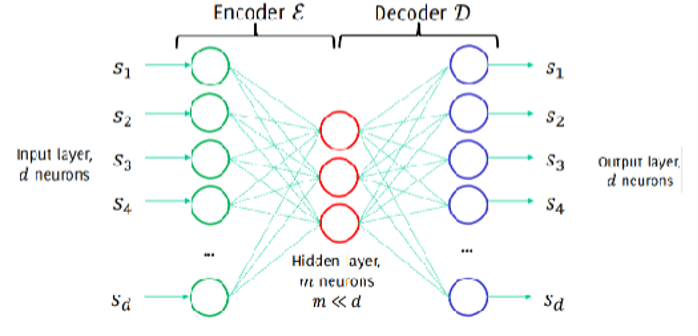
\includegraphics[width=0.5\linewidth]{img/lecture24/Picture11.png}
    \caption{Structure of an autoencoder used for reconstruction-based anomaly detection.}
    \label{fig:autoencoder}
\end{figure}

During training, the network is optimized to reconstruct all samples in the
training set. The reconstruction loss over the training data is given by
\[
L(\mathcal{T}_R)=\sum_{s\in\mathcal{T}_R}\|s-D(E(s))\|_2.
\]
Training is performed using standard backpropagation and stochastic gradient
descent. After training, anomalies are detected by identifying samples whose
reconstruction error is significantly larger than that observed on the normal
training data.

\subsubsection{Gradient-Based Regularization}

Recent work has shown that reconstruction alone may not always guarantee strong
separation between normal and anomalous data. Gradient-based regularization
techniques address this issue by constraining how the model behaves in regions
of the input space that are likely to contain anomalies.

One example is Gradient Constrained Optimization (GradCON), which penalizes
model updates that reduce reconstruction error for samples suspected to be
anomalous. Intuitively, this encourages the model to remain highly specialized
for normal data and prevents it from generalizing too well to abnormal inputs.
Such regularization improves the separability of reconstruction errors and
leads to more reliable anomaly detection.

\subsubsection{Ensemble and Multi-Scale Detection}

In real-world systems, anomaly detection often benefits from combining multiple
complementary signals. Ensemble approaches integrate reconstruction-based
scores with methods such as Maximum Softmax Probability, patch-based analysis,
and manifold learning. By aggregating anomaly scores across multiple feature
scales and modeling assumptions, these systems achieve improved robustness and
reduced false positive rates.

Hybrid pipelines that combine statistical models, deep neural networks, and
ensemble scoring represent the current state of the art in large-scale anomaly
detection systems.

% \section{Q\&A Section}

% \begin{enumerate}
%     \item What is the primary challenge in defining anomalies within a dataset?\newline
    
%     \textbf{Answer:} The primary challenge is accurately defining ``normal" behavior within the data. Since anomalies are identified based on deviations from normal patterns, an unclear or incorrect definition of normality can lead to either false positives (normal data misclassified as anomalies) or false negatives (anomalies classified as normal). 
%     \newline
    
%     \textbf{Explanation:} The process of anomaly detection relies heavily on understanding the statistical properties of normal data. In many cases, normal behavior can vary significantly across contexts, requiring careful consideration of the domain, data patterns, and use case. This challenge underscores the importance of robust statistical modeling or machine learning techniques.\newline

%     \item Why are anomalies often considered the most significant data points in a dataset? \newline
    
%     \textbf{Answer:} Anomalies typically highlight rare and unusual events that may signal critical insights or important occurrences, such as fraudulent transactions, system failures, or medical conditions.\newline 
    
%     \textbf{Explanation:} While anomalies represent only a small fraction of the data, they are often highly informative because they stand out from the background of normal behavior. This makes them valuable in applications where detecting rare events can have substantial impacts, such as cybersecurity or medical diagnostics.\newline

%     \item What are the two main components of an anomaly detection algorithm in a statistical framework? \newline
    
%     \textbf{Answer:} The two main components are (1)Statistic: A measurement that quantifies the behavior of the data and responds predictably under normal conditions, and (2) Decision Rule: A mechanism to interpret the statistic and classify data points as normal or anomalous. \newline 
    
%     \textbf{Explanation:} The statistic provides a mathematical or computational representation of the data's characteristics, while the decision rule applies thresholds or confidence intervals to make a binary decision (normal vs. anomalous). Together, these components form the foundation for statistical anomaly detection.\newline

%     \item What is the trade-off between the True Positive Rate (TPR) and False Positive Rate (FPR) in anomaly detection?\newline 
    
%     \textbf{Answer:} There is an inherent trade-off where lowering the threshold parameter ($\gamma$) increases TPR (detecting more anomalies) but also raises FPR (increasing false positives). Conversely, raising $\gamma$ reduces FPR but may lower TPR, leading to missed anomalies.\newline
%     \textbf{Explanation:} The threshold $\gamma$ determines the sensitivity of the anomaly detection algorithm. Adjusting $\gamma$ too low makes the model more inclusive, detecting more anomalies but potentially misclassifying normal points as anomalies. A higher threshold does the opposite, making the model more conservative.\newline

%     \item What is the main challenge of density-based methods in anomaly detection?\newline
    
%     \textbf{Answer:} The main challenge is handling high-dimensional data, as estimating probability density functions (PDFs) in high dimensions is computationally expensive and prone to overfitting.
%     \newline
    
%     \textbf{Explanation:} Density-based methods rely on accurate modeling of the normal data distribution, but as dimensionality increases, data sparsity and computational complexity make it difficult to achieve robust estimations. This is often referred to as the "curse of dimensionality."\newline
    
%     \item What are the primary advantages of using the optimization techniques discussed in the lecture for reducing computational overhead in neural networks? \newline
    
%     \textbf{Answer:} The optimization techniques such as quantization, pruning, and knowledge distillation help in:
%     Reducing model size - These techniques decreases the memory footprint, making models feasible for edge devices.
%     Improving inference speed - By simplifying computations, these methods ensure faster inference without significant loss of accuracy. 
%     Energy efficiency - Optimization reduces power consumption, which is critical for deploying models on mobile or IoT devices. \newline 
    
%     \textbf{Explanation:} Quantization reduces the precision of the weights and activations, thereby lowering the computational requirements. Pruning removes redundant parameters, maintaining the key structure of the model while improving efficiency. Knowledge distillation transfers knowledge from a larger ``teacher" model to a smaller ``student" model, maintaining performance while reducing complexity.
    
%     \item Explain the role of gradient clipping in addressing exploding gradients during backpropagation through time (BPTT) in RNNs. \newline 
    
%     \textbf{Answer:} Gradient clipping restricts the magnitude of gradients to a predefined threshold during the backpropagation process. If a gradient's norm exceeds this threshold, it is scaled down proportionally to fit within the limit. \newline 
    
%     \textbf{Explanation:} In RNNs, gradients can grow exponentially during BPTT, leading to numerical instability and poor convergence (exploding gradients). Gradient clipping ensures stable training by preventing gradients from becoming excessively large. It acts as a safeguard, especially in deep networks where long-term dependencies are critical but prone to instability.
    
%     \item What is the significance of attention mechanisms in transformers compared to traditional RNN-based sequence models? \newline 
    
%     \textbf{Answer:} Attention mechanisms allow models to focus on relevant parts of the input sequence dynamically, rather than relying solely on sequential processing like RNNs. This improves parallelism and efficiency. \newline 
    
%     \textbf{Explanation:} RNNs process sequences step-by-step, making them computationally expensive for long inputs. Attention mechanisms, a core component of transformers, compute relationships between all parts of the sequence simultaneously. This approach enhances the ability to capture long-term dependencies, enabling state-of-the-art performance in tasks like machine translation and text summarization.

%     \item How does the choice of activation function affect the training dynamics and expressiveness of a neural network? \newline 
    
%     \textbf{Answer:} The activation function determines the network's ability to capture non-linear relationships and influences gradient propagation during backpropagation. \newline
    
%     \textbf{Explanation:} ReLU (Rectified Linear Unit) is commonly used due to its simplicity and efficiency, avoiding vanishing gradient issues seen in sigmoid and tanh. However, ReLU can suffer from "dead neurons." Alternatives like Leaky ReLU and GELU address these issues by allowing small gradients for negative inputs, improving learning dynamics and overall expressiveness.
    
%     \item What are the trade-offs involved in using batch normalization for stabilizing training in deep networks? \newline
    
%     \textbf{Answer:} Batch normalization accelerates training by normalizing intermediate layer outputs, reducing internal covariate shift. However, it introduces computational overhead and can cause issues during inference when batch statistics differ from training statistics. \newline 
    
%     \textbf{Explanation:} During training, batch normalization reduces sensitivity to weight initialization and learning rates. However, it relies on batch statistics, which can vary significantly for small batch sizes or during inference, potentially affecting performance. Despite these challenges, its ability to stabilize training often outweighs the drawbacks.
% \end{enumerate}

\section{Q\&A Section}

\begin{enumerate}

\item What is the primary challenge in defining anomalies within a dataset?\newline
\textbf{Answer:} The primary challenge is accurately defining ``normal'' behavior. Since anomalies are detected as deviations from normal patterns, an incorrect definition of normality can lead to false positives or false negatives.\newline
\textbf{Explanation:} Anomaly detection relies on modeling the statistical properties of normal data. If the model of normal behavior is inaccurate or incomplete, the detection process becomes unreliable.

\item Why are anomalies often considered the most significant data points in a dataset?\newline
\textbf{Answer:} Anomalies correspond to rare and unusual events such as fraud, failures, or medical abnormalities.\newline
\textbf{Explanation:} Although rare, anomalies often carry the most actionable information and are therefore critical in many real-world applications.

\item What are the two main components of a statistical anomaly detection algorithm?\newline
\textbf{Answer:} (1) A statistic that measures data behavior, and (2) a decision rule that determines whether a sample is anomalous.\newline
\textbf{Explanation:} The statistic quantifies how unusual a sample is, while the decision rule applies a threshold to classify it as normal or anomalous.

\item What is the trade-off between True Positive Rate (TPR) and False Positive Rate (FPR)?\newline
\textbf{Answer:} Lowering the threshold $\gamma$ increases TPR but also increases FPR, while raising $\gamma$ decreases FPR but may miss anomalies.\newline
\textbf{Explanation:} Threshold selection determines the sensitivity of the detector and directly affects detection performance.

\item What is the main challenge of density-based anomaly detection methods?\newline
\textbf{Answer:} Density estimation becomes difficult in high-dimensional spaces due to the curse of dimensionality.\newline
\textbf{Explanation:} As dimensionality increases, data become sparse and probability density estimation becomes computationally expensive and prone to overfitting.

\item Why is unsupervised anomaly detection often formulated as a ranking problem?\newline
\textbf{Answer:} Because models typically output anomaly scores rather than class labels.\newline
\textbf{Explanation:} Samples are ranked by their anomaly score, and the most abnormal samples are flagged based on a threshold or top-$k$ selection.

\item Why are anomalies easier to detect using Isolation Forest compared to density estimation?\newline
\textbf{Answer:} Anomalies are easier to isolate and require fewer random splits in decision trees.\newline
\textbf{Explanation:} Isolation Forest exploits the fact that anomalous points are rare and different, leading to shorter path lengths during recursive partitioning.

\item Why do reconstruction-based methods detect anomalies using reconstruction error?\newline
\textbf{Answer:} Models trained on normal data reconstruct normal samples well but fail to reconstruct anomalies.\newline
\textbf{Explanation:} Large reconstruction errors indicate that the input does not lie on the learned manifold of normal data.

\item Why is Maximum Softmax Probability (MSP) useful for detecting out-of-distribution samples?\newline
\textbf{Answer:} Out-of-distribution inputs typically produce lower softmax confidence scores.\newline
\textbf{Explanation:} Neural networks tend to assign high probability to familiar data and lower confidence to unfamiliar inputs.

\item Why is anomaly detection challenging in high-dimensional data?\newline
\textbf{Answer:} Distance and density measures become less informative in high dimensions.\newline
\textbf{Explanation:} This phenomenon, known as the curse of dimensionality, makes it harder to distinguish normal and anomalous samples reliably.

\end{enumerate}


\end{document}

